\documentclass[11pt]{article}

\usepackage[a4paper, margin=2cm, top=1.5cm]{geometry}
\usepackage{amsmath, amssymb}
\usepackage{booktabs}
\usepackage{enumitem}
\usepackage{tikz}
\usepackage[colorlinks, urlcolor=blue, linkcolor=red]{hyperref}

\usetikzlibrary{arrows.meta, positioning}

\DeclareMathOperator{\Poiss}{Poiss}
\newcommand{\Gam}{\mathcal{G}}

\title{Seminar 1. Bayesian Reasoning}
\author{Bayesian Methods}
\date{}

\begin{document}

\maketitle
\vspace{-2em}

\begin{enumerate}[label=\arabic*.]

\item A medical test finds a serious disease in a patient. The test is
  99\% accurate: if the patient has the disease, the test is positive with
  probability 99\%; if the patient does not have the disease, the test is
  negative with probability 99\%. The disease is rare: only one person in
  10\,000 has it. Find the probability that the patient really has the
  disease.

\item Consider the following probabilistic model. At a seminar, a student
  answers badly ($A = 1$) or well ($A = 0$). This depends on whether the
  student has depression ($D = 1$ or $D = 0$) and whether the student went
  to a party the night before ($P = 1$ or $P = 0$). The party can also give
  the student a headache ($H = 1$). A bad answer makes the teacher unhappy
  ($T = 1$). Figure~\ref{fig:model} shows the causal relations in the model.
  The probabilities are:
  \begin{center}
    \begin{tabular}[t]{c|cc}
      \toprule
      $p(A = 1 \mid P, D)$ & $P$ & $D$ \\
      \midrule
      0.999 & 1 & 1 \\
      0.9   & 1 & 0 \\
      0.9   & 0 & 1 \\
      0.01  & 0 & 0 \\
      \bottomrule
    \end{tabular}
    \quad
    \begin{tabular}[t]{c|c}
      \toprule
      $p(H = 1 \mid P)$ & $P$ \\
      \midrule
      0.9 & 1 \\
      0.2 & 0 \\
      \bottomrule
    \end{tabular}
    \quad
    \begin{tabular}[t]{c|c}
      \toprule
      $p(T = 1 \mid A)$ & $A$ \\
      \midrule
      0.95 & 1 \\
      0.5  & 0 \\
      \bottomrule
    \end{tabular}

    \medskip
    $p(P = 1) = 0.2, \qquad p(D = 1) = 0.4.$
  \end{center}
  Find $p(P = 1 \mid H = 1)$, $p(P = 1 \mid T = 1)$, and
  $p(P = 1 \mid T = 1, H = 1)$.

\item Let $x_1 \sim \Poiss(\lambda_1)$ and $x_2 \sim \Poiss(\lambda_2)$ be
  two independent Poisson random variables, that is,
  $p(x_i = k) = \exp(-\lambda_i) \frac{\lambda_i^k}{k!}$,
  $k = 0, 1, 2, \ldots$ Prove that
  $x_1 + x_2 \sim \Poiss(\lambda_1 + \lambda_2)$.

\item Let $x_1, x_2, \ldots, x_N$ be an independent sample from
  $\Poiss(\lambda)$. Find the maximum likelihood estimate of $\lambda$.

\item Let $x_1, x_2, \ldots, x_N$ be an independent sample from
  $\Poiss(\lambda)$. The prior distribution is the gamma distribution
  \[
    p(\lambda) = \Gam(\lambda \mid a, b)
    = \frac{b^a}{\Gamma(a)} \lambda^{a - 1} \exp(-b \lambda),
    \quad a, b > 0.
  \]
  Find the Bayesian estimate of $\lambda$ as the mean of the posterior
  distribution $p(\lambda \mid x_1, \ldots, x_N)$.

\end{enumerate}

\begin{figure}[ht]
  \centering
  \vspace{-1em}
  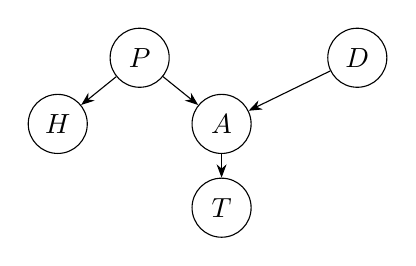
\begin{tikzpicture}[
      node distance=0.3cm and 0.5cm,
      var/.style={circle, draw, minimum size=0.75cm},
      >={Stealth},
    ]
    \node[var] (P) {$P$};
    \node[var, right=2cm of P] (D) {$D$};
    \node[var, below left=of P] (H) {$H$};
    \node[var, below right=of P] (A) {$A$};
    \node[var, below=of A] (T) {$T$};
    \draw[->] (P) -- (H);
    \draw[->] (P) -- (A);
    \draw[->] (D) -- (A);
    \draw[->] (A) -- (T);
  \end{tikzpicture}
  \caption{Causal relations for Problem~2}
  \label{fig:model}
\end{figure}

\paragraph{Notes on comparing the estimates from Problems 4 and 5.}

\begin{enumerate}[label=\arabic*.]
  \item For more about non-informative priors, see Section~5.4 ``Priors''
    in Kevin P.\ Murphy, \emph{Machine Learning: A Probabilistic
    Perspective}.
  \item The prior $p(\lambda) \propto \frac{1}{\lambda}$ is a uniform prior
    on $\log \lambda$. To see this, use the change-of-variables rule for
    the density of a function of a random variable. See, for example,
    \href{https://en.wikipedia.org/wiki/Probability_density_function#Function_of_random_variables_and_change_of_variables_in_the_probability_density_function}{this
    article}.
\end{enumerate}

\end{document}
